\documentclass[ENG]{TFUOC}

\usepackage{graphicx}
\usepackage{float}
\usepackage{tikz}
\usepackage{booktabs}
\usepackage{array}
\usepackage{multirow}
\usetikzlibrary{arrows.meta,shapes.geometric,positioning,fit,backgrounds,calc}

%Introduce Work Data
\title{Analítica avanzada sobre datos de plataformas VOD y generadores de contenidos en redes sociales}
\titcrt{Analítica de plataformas VOD} %Short title to appear in header
\author{Pablo Jiménez Cruz}
\date{March 1, 2026}


\nomPDC{Francesc Julbe López}
\nomPRA{Appoint Responsible Teaching Staff}
\titulac{Master in Data Science}
\area{Data Science}
\idioma{English}
\credits{12}
\parcla{artificial intelligence, data analytics, video-on-demand platforms, multimodal content generation, social media analytics, automatic speech recognition, short-form video}

\licenc{ccBy}

%%%%%%%%%%
% Summary in language

\abstractenglish{
The rapid growth of Video-on-Demand (VOD) platforms and social media ecosystems has generated large volumes of audiovisual and audience-related data, creating new opportunities for data-driven content production. However, existing analytical and content-generation tools remain fragmented, limiting their effective use, particularly for small and medium-scale creators.

This Final Master's Project presents the design and development of a modular artificial intelligence platform integrating data ingestion, advanced analytics, and automated audiovisual content generation. The system combines data extracted from the YouTube Data API~v3 with natural language processing, multimodal analysis, and machine learning techniques to transform dispersed data into actionable insights.

The adopted methodology follows an incremental and modular development approach, where independent components are progressively implemented and validated before integration into a unified architecture built on FastAPI, PostgreSQL, and a React single-page application. The platform covers data ingestion and structured storage, internal performance analysis, automatic video segmentation for short-form content generation, multilingual subtitle creation, and multimodal content summarization powered by large language models.

Results demonstrate the feasibility of automating key stages of the audiovisual production workflow while enabling quantitative evaluation through performance metrics such as click-through rate, audience retention, and viewing time. The proposed architecture improves efficiency, scalability, and decision-making capabilities in digital content production environments, and an economic analysis confirms its viability as a deployable SaaS product.
}

\begin{document}

\estructura

\tableofcontents

\listoffigures

\listoftables


%==========================================================
\chapter{Introduction}
%==========================================================

\section{Context and justification of the project}

Over the last decade, the digital audiovisual landscape has undergone a profound structural transformation. The consolidation of Video-on-Demand platforms such as YouTube, together with the rapid expansion of short-form video formats (Shorts, Reels, TikTok), has reshaped how audiovisual content is produced, distributed, and monetized \cite{vod_bigdata}. YouTube alone reports more than 500 hours of video uploaded every minute, generating an enormous volume of structured metadata, audience interaction records, and engagement signals that remain largely underexploited by independent creators \cite{recommender_systems_streaming}.

The current content economy is driven by algorithmic recommendation systems, attention-based monetization models, and highly dynamic market trends \cite{recommender_systems_streaming}. In this environment, creators and production teams compete not only on creative quality, but also on their capacity to interpret platform data, detect trends, and optimize content performance in near real-time. Official services such as the YouTube Data API~v3 and YouTube Analytics API provide access to large volumes of structured engagement data; however, the systematic exploitation of these datasets remains limited.

Existing tools are typically fragmented: independent dashboards, clipping utilities, subtitle generators, or trend trackers that operate in isolation without interoperability or analytical feedback integration. This fragmentation creates measurable inefficiencies. Small and medium-sized creators lack access to advanced data-driven workflows, while larger production environments rely on costly proprietary solutions.

There is therefore a clear opportunity to design an integrated platform capable of: (i)~extracting and structuring relevant data from VOD platforms through official APIs; (ii)~transforming that data into actionable market intelligence via machine learning models; (iii)~automating content repurposing processes based on analytical evidence; and (iv)~incorporating performance feedback for iterative optimization.

This Final Master's Project proposes the design and implementation of \textit{youtube-suite}, a modular artificial intelligence system integrating data ingestion, advanced analytics, and automated content generation within a unified workflow. The proposal aligns with current research in data-driven media production, computational social science, and AI-assisted creativity, where multimodal analysis and feedback loops are applied to optimize content strategy and audience impact \cite{ai_content_creation}.

Figure~\ref{fig:architecture} illustrates the layered architecture of the proposed system, organized according to clean architecture principles with clearly separated concerns across four layers.

\begin{figure}[H]
\centering
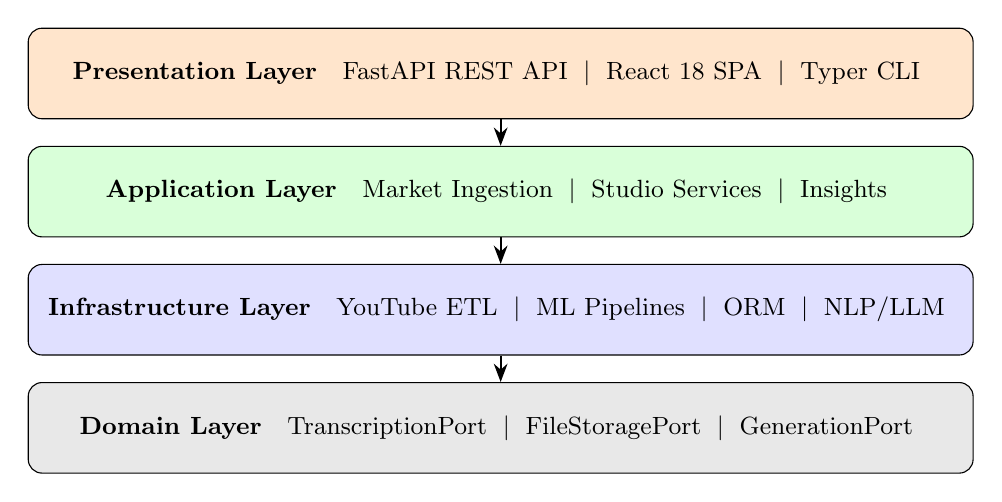
\begin{tikzpicture}[
    layer/.style={draw, rounded corners=5pt, minimum width=12cm, minimum height=1.15cm,
                  align=center, font=\small},
    sublabel/.style={font=\scriptsize\itshape}
]
\node[layer, fill=orange!20] (pres) at (0,4.5) {
    \textbf{Presentation Layer}\quad
    FastAPI REST API \;$\vert$\; React~18 SPA \;$\vert$\; Typer CLI
};
\node[layer, fill=green!15] (app) at (0,3.0) {
    \textbf{Application Layer}\quad
    Market Ingestion \;$\vert$\; Studio Services \;$\vert$\; Insights
};
\node[layer, fill=blue!12] (infra) at (0,1.5) {
    \textbf{Infrastructure Layer}\quad
    YouTube ETL \;$\vert$\; ML Pipelines \;$\vert$\; ORM \;$\vert$\; NLP/LLM
};
\node[layer, fill=gray!18] (domain) at (0,0.0) {
    \textbf{Domain Layer}\quad
    TranscriptionPort \;$\vert$\; FileStoragePort \;$\vert$\; GenerationPort
};
\draw[-Stealth,thick] (pres.south) -- (app.north);
\draw[-Stealth,thick] (app.south) -- (infra.north);
\draw[-Stealth,thick] (infra.south) -- (domain.north);
\end{tikzpicture}
\caption{Layered architecture of the \textit{youtube-suite} platform following clean architecture principles.}
\label{fig:architecture}
\end{figure}

%--------------------------------------------------
\section{Objectives of the project}

\subsection*{General objective}

To design and implement a modular artificial intelligence platform capable of integrating data ingestion, advanced analytics, and automated audiovisual content generation for VOD environments, exposed through a unified API and a web-based user interface.

\subsection*{Specific objectives}

\begin{enumerate}
\item Develop a scalable data extraction pipeline using the YouTube Data API~v3 with quota-aware orchestration and idempotent storage.
\item Design and implement a structured PostgreSQL database with three domain schemas (\textit{market}, \textit{studio}, \textit{app}) supporting both historical and time-series data.
\item Build internal analytics modules focused on platform-specific performance indicators (click-through rate, views, engagement).
\item Implement external market analysis tools for trend detection and keyword monitoring.
\item Develop an automated Video-to-Shorts pipeline combining automatic speech recognition, speaker diarization, semantic segmentation, and multi-factor highlight scoring.
\item Implement a subtitle generation and multilingual correction module based on automatic speech recognition.
\item Design a multimodal description generation system leveraging large language models and SEO trend signals.
\item Expose all functionality through a documented REST API and an interactive React frontend.
\item Define and apply quantitative evaluation metrics for performance assessment of the generated content.
\item Conduct an economic evaluation of the project assessing development costs, operational costs, and viability.
\end{enumerate}

%--------------------------------------------------
\section{Impact on sustainability, ethical-social aspects and diversity}
\label{s:etic}

This project integrates the Competence of Ethical and Global Commitment (CCEG) following the transversal guidelines for Final Projects. The reflection is structured around the three required dimensions.

\subsection*{Sustainability}

The main environmental impact derives from the computational resources required for data processing, storage, and AI model execution, particularly for automatic speech recognition and speaker diarization. These activities carry energy and infrastructure costs aligned with ODS~9 (Industry, Innovation and Infrastructure) and ODS~12 (Responsible Consumption and Production).

To mitigate this impact, the system applies several efficiency criteria: periodic rather than continuous API polling; reuse of generated artefacts such as transcripts and embeddings across pipeline stages; chunked audio processing to avoid redundant computation; and containerization via Docker to ensure reproducible, controlled resource usage. These decisions reduce both computational overhead and storage footprint without sacrificing analytical quality.

\subsection*{Ethical behaviour and social responsibility}

The platform operates exclusively with publicly available data obtained through official YouTube APIs, respecting platform terms of service and applicable data protection regulations (GDPR). A latent risk lies in the possibility of optimizing content purely for engagement metrics or generating decontextualized fragments through automated clipping tools.

To address this, the system is conceived as a decision-support tool: all generated content (clips, subtitles, descriptions) requires human supervision before publication. Scoring weights for the highlight detection module are configurable and exposed in the user interface, allowing creators to privilege content quality over algorithmic proxies of engagement. This design contributes to ODS~8 (Decent Work and Economic Growth) by empowering creators with advanced analytical capabilities while promoting responsible use of AI.

\subsection*{Diversity, gender and human rights}

Automatic speech recognition and language model outputs may reflect biases present in training data. This risk has been considered in the design of subtitle generation and description synthesis, both of which expose outputs to human validation before use.

A positive impact of the platform lies in improved accessibility: multilingual subtitle generation facilitates access for users with hearing impairments and for diverse linguistic communities. Language localization of LLM prompts (supporting Spanish, English, French, German, Portuguese, Italian, Japanese, Korean, and Chinese) reinforces content democratization, contributing to ODS~5 (Gender Equality) and ODS~10 (Reduced Inequalities).

%--------------------------------------------------
\section{Approach and method followed}

The project follows a modular incremental development methodology structured into four progressive phases, where each component is validated independently before integration.

\textbf{Phase 1 — Data Ingestion.} Implementation of API connectors to extract structured data from the YouTube Data API~v3. This phase includes authentication management, API quota optimization, and idempotent data loading into PostgreSQL.

\textbf{Phase 2 — Storage and Structuring.} Design of a relational schema in PostgreSQL organized across three schemas: \textit{market} for catalog and audience data, \textit{studio} for creator assets and generated artefacts, and \textit{app} for operational job state. Time-series snapshots of engagement metrics enable longitudinal analysis.

\textbf{Phase 3 — Analytical Modeling.} Development of internal analytics (engagement KPI aggregation), external trend detection (keyword extraction from high-view titles), and semantic pipelines (sentence embeddings for content segmentation).

\textbf{Phase 4 — Content Generation.} Implementation of AI-based tools: the Video-to-Shorts pipeline (ASR, diarization, scoring), the subtitle generation module (faster-whisper), and the multimodal description generator (Claude API with SEO keyword injection).

This incremental approach minimizes systemic risk and allows controlled experimentation at each integration boundary. Independent validation of each module was performed before assembling the unified platform.

%--------------------------------------------------
\section{Planning of the project}

The development schedule aligns directly with the four methodological phases:

\begin{itemize}
\item \textbf{Weeks 1–2} (Feb.~18 – Mar.~1): Architectural definition, environment setup, and Phase~1 design.
\item \textbf{Weeks 3–4} (Mar.~2 – Mar.~15): Implementation of YouTube API connectors and PostgreSQL schema (Phases~1–2).
\item \textbf{Weeks 5–6} (Mar.~16 – Mar.~29): Development of market analytics and insights modules (Phase~3).
\item \textbf{Weeks 7–8} (Mar.~30 – Apr.~12): Implementation of the Video-to-Shorts pipeline (Phase~4).
\item \textbf{Weeks 9–10} (Apr.~13 – Apr.~26): Subtitle generation and multilingual processing module.
\item \textbf{Weeks 11–12} (Apr.~27 – May~10): Multimodal description generator and React frontend.
\item \textbf{Weeks 13–14} (May~11 – May~25): Experimental validation, integration testing, and documentation.
\end{itemize}

Identified risks include YouTube API quota constraints, evolving platform policies, and integration complexity between heterogeneous ML models. These are mitigated through modular development, staged testing, and controlled evaluation environments using representative video datasets.

%--------------------------------------------------
\section{Brief summary of the products obtained}

The outcome of this project is \textit{youtube-suite}: a unified monorepo organized as a deployable software platform. The principal artefacts produced are the following.

\textbf{Market data pipeline.} A fully orchestrated ETL pipeline extracting video metadata, engagement statistics, comments, and trending content from the YouTube Data API~v3. Data are stored in a PostgreSQL database with time-series support for longitudinal analysis.

\textbf{Analytics and insights modules.} Internal KPI aggregation (total views, top videos, category distribution, views over time) and external trend detection via keyword extraction from high-performing video titles.

\textbf{Video-to-Shorts pipeline.} An end-to-end automatic short-form content generation system combining FFmpeg-based audio extraction, WhisperX speech recognition with word-level alignment, pyannote speaker diarization, sentence-level semantic segmentation via SBERT embeddings, and a multi-factor scoring model based on a Random Forest classifier.

\textbf{Subtitle generation module.} A chunked ASR pipeline based on faster-whisper producing SRT subtitle files with optional FFmpeg-based subtitle embedding directly into the video stream.

\textbf{Multimodal description generator.} An LLM-based system that synthesizes SEO-optimized video descriptions from transcript content and trending keyword signals, with support for both the Anthropic Claude API and a local Ollama deployment.

\textbf{Unified REST API and web interface.} A FastAPI application exposing all pipeline functionality through standardized, documented endpoints, complemented by a React~18 single-page application for interactive asset management, job monitoring, and results visualization.

\textbf{Containerized infrastructure.} A Docker Compose configuration providing PostgreSQL and the API service in a reproducible, portable deployment environment.

%--------------------------------------------------
\section{Brief description of the other chapters of the report}

Chapter~2 reviews the state of the art in VOD analytics and automated audiovisual content generation, covering data ingestion architectures, recommendation systems, highlight detection models, and automatic speech translation.

Chapter~3 describes the materials, methods, and design decisions adopted during development, including the technology stack, database architecture, pipeline implementations, and an economic evaluation of the project.

Chapter~4 presents the experimental results and quantitative evaluation of the developed tools.

Chapter~5 discusses conclusions, limitations, objective achievement, and future research directions.

%--------------------------------------------------
\section{Statement on the use of generative artificial intelligence}

Generative artificial intelligence tools (specifically large language models) were used as productivity aids during the ideation phase, documentation structuring, code prototyping, and linguistic refinement of technical writing.

Their use was limited to: (i)~draft structuring and grammar assistance; (ii)~rapid prototyping support for boilerplate code; and (iii)~comparative exploration of architectural alternatives. All generated content was critically reviewed, validated, and substantially adapted prior to inclusion. Architectural design, implementation decisions, experimental configuration, and validation remain entirely the responsibility of the author.

The use of generative AI tools followed institutional guidelines and supervisory awareness, ensuring intellectual ownership and academic integrity.


%==========================================================
\chapter{State of the Art in VOD Analytics and Audiovisual Content Generation}
%==========================================================

The video-on-demand (VOD) ecosystem is increasingly driven by large-scale data analytics and artificial intelligence. Modern streaming platforms collect massive volumes of user interaction data, including viewing habits, engagement patterns, and audience preferences. These data underpin recommendation algorithms and content strategy decisions at industrial scale \cite{vod_bigdata, recommender_systems_streaming}.

Personalized recommendation systems are central to the business model of major platforms. Research by Covington et al.\ \cite{recommender_systems_streaming} demonstrates a two-stage deep neural network architecture for YouTube recommendations operating at the scale of hundreds of millions of users, relying on watch history, search queries, and demographic signals. Similarly, Gomez-Uribe and Hunt \cite{vod_bigdata} report that approximately 80 per cent of total viewing time on Netflix is attributable to its recommendation engine, highlighting the direct link between data-driven content discovery and platform revenue. These findings establish the quantitative importance of engagement metrics such as watch time, audience retention, and click-through rate as primary optimization targets for content producers.

\section{Data Ingestion and Storage}

Most major VOD platforms expose developer APIs that allow structured retrieval of video metadata, performance statistics, and audience interaction data. The YouTube Data API~v3, the primary data source in this project, provides endpoints for video metadata, trending content retrieval by geographic region (via the \texttt{chart=mostPopular} parameter), channel information, and comment threads.

Recent research demonstrates how systematic API-based data collection enables large-scale analytics. Gytlid et al.\ \cite{gytlid2025} illustrate a multi-country trending video collection methodology, where videos are periodically retrieved for each geographic region and stored with their associated engagement statistics and textual metadata. The resulting time-series datasets support cross-cultural analysis of content trends and audience behavior.

Architecturally, collected data are typically ingested into relational or columnar storage systems that support both point-in-time queries and longitudinal aggregation. The Extract-Transform-Load (ETL) pattern, supplemented by idempotent upserts, is the standard approach for maintaining consistency across incremental ingestion cycles \cite{vod_bigdata}. These patterns underpin the data pipeline implemented in this project.

\section{Internal Performance Analysis}

Once collected and stored, internal analytics can evaluate content performance through platform-specific KPIs. Key indicators on YouTube include audience retention curves, click-through rate (CTR), average view duration, and engagement rate (likes, shares, and comments normalized by views). These metrics determine both creator revenue and algorithmic promotion within the platform.

Academic studies emphasize that the systematic analysis of these indicators is essential for content strategy optimization. Variables such as video length, publication schedule, thumbnail design, and topic selection can significantly influence audience engagement and recommendation ranking \cite{vod_bigdata}. Predictive models trained on historical engagement data can forecast the performance of newly published content, enabling creators to refine editorial decisions before publication.

Time-series analysis of engagement metrics is particularly valuable for detecting changes in audience behavior, seasonal trends, and the impact of content format experiments. The storage architecture must therefore support efficient temporal queries at both video and channel granularity.

\section{External Trend Detection}

While internal platform data provide valuable performance signals, understanding broader social trends requires analyzing content from external sources. Social media platforms contain large volumes of user-generated text reflecting emerging topics, public discourse, and cultural dynamics.

Natural language processing techniques are widely applied to transform unstructured social data into actionable intelligence. Methods including sentiment analysis, named entity recognition, and topic modeling allow researchers to detect trending subjects and monitor public opinion \cite{singh2025, social_media_nlp}. The combination of word frequency analysis and temporal aggregation enables the identification of keywords that are gaining traction before they reach mainstream platform search queries.

Integrating these external signals with internal performance data remains a recognized challenge. A unified analytical pipeline combining both sources would provide a more comprehensive understanding of audience demand and support more accurate content planning. The current project addresses this integration by extracting keywords from high-view video titles within the platform database as a lightweight trend signal, complementing the full market ingestion pipeline.

\section{Automatic Generation of Audiovisual Content}

\subsection*{Video summarization and highlight detection}

Automatic video summarization aims to produce a condensed representation of a longer video by selecting the most relevant segments. Saini et al.\ \cite{video_summarization_review} distinguish between static summaries (keyframe sets) and dynamic summaries (video skimming), where the latter preserve temporal continuity and are better suited to short-form content platforms.

State-of-the-art highlight detection approaches rely on deep learning architectures combining convolutional and sequential components. Kwak et al.\ \cite{spot_model} propose a hybrid model combining convolutional neural networks with temporal transformer attention to detect highlights in long videos: the convolutional layers capture local visual features, while the transformer models long-range temporal dependencies. Experimental results show that this hybrid architecture significantly outperforms earlier transformer-only baselines on standard benchmark datasets.

An alternative approach exploits implicit audience interaction signals. Some platforms expose replay frequency data indicating which segments viewers replay most often; these signals can be used as weak supervision labels for highlight detection models, since repeated viewing correlates with subjective engagement \cite{video_highlight_detection}.

In this project, highlight detection is reformulated as a text-based task: semantic segmentation of transcripts using sentence embeddings, combined with audio energy analysis, speaker change detection, and hook phrase identification, provides a multimodal signal that does not require visual feature extraction and operates efficiently on CPU hardware.

\subsection*{Automatic speech recognition and subtitle generation}

Automatic speech recognition (ASR) has undergone a major quality inflection with the release of Whisper \cite{radford2023whisper}, a large-scale weakly supervised model trained on 680,000 hours of multilingual audio. Whisper achieves near-human accuracy across a wide range of accents, noise conditions, and languages, and is available in multiple size configurations allowing deployment at different computational budgets.

WhisperX \cite{bain2023whisperx} extends Whisper with forced phoneme alignment, producing word-level timestamps with higher precision — a critical requirement for clip boundary computation in the Video-to-Shorts pipeline. The faster-whisper implementation \cite{fasterwhisper} provides an optimized inference backend using CTranslate2 quantization, enabling CPU-friendly deployment without significant accuracy degradation.

More recent research explores end-to-end speech translation directly to subtitle format, bypassing intermediate transcription-translation pipelines \cite{papi2023}. Such architectures reduce error propagation between stages. For this project, language-specific transcription followed by LLM-based refinement provides a practical balance between accuracy and deployment complexity.

\subsection*{Speaker diarization}

Speaker diarization assigns speech segments to individual speakers, enabling the system to identify speaker turns within a conversation. The pyannote.audio framework \cite{bredin2021pyannote} provides a modular neural pipeline for end-to-end diarization, combining voice activity detection, speaker embedding extraction, and clustering. The \texttt{speaker-diarization-3.1} model achieves state-of-the-art performance on standard benchmarks and is used in this project to annotate transcript segments with speaker identities.

\section{Multimodal Content Generation}

An emerging research direction focuses on AI-assisted generation of textual and audiovisual content accompanying video publications. Li et al.\ \cite{ai_content_creation} survey the application of AI across multiple stages of the content creation process, including topic identification, metadata generation, and promotional material synthesis.

Large language models (LLMs) have become the primary tool for text generation tasks in this context. Their capacity to condition output on transcript content, keyword lists, and platform-specific style requirements makes them well-suited to automated description generation. SEO-informed prompting strategies, where trending keywords are injected into generation prompts, have been adopted by several content optimization platforms to improve discoverability without sacrificing natural language quality.

\section{Semantic Text Embeddings}

Sentence-level semantic embeddings are a fundamental component of the content segmentation pipeline. Reimers and Gurevych \cite{reimers2019sbert} introduce Sentence-BERT (SBERT), a modification of the BERT architecture that uses siamese and triplet networks to produce semantically meaningful fixed-dimensional sentence representations. SBERT embeddings support efficient cosine similarity computation and are applied in this project to detect topic shift boundaries between consecutive transcript segments. The \texttt{all-mpnet-base-v2} model, which achieves strong performance on semantic textual similarity benchmarks, is used as the default embedding backbone.

\section{Conclusions}

The state of the art in VOD analytics and audiovisual content generation reveals a highly data-driven ecosystem in which large-scale data infrastructures, machine learning models, and artificial intelligence techniques are deeply integrated.

Three principal trends emerge. First, personalized recommendation systems constitute the primary mechanism driving user engagement and content discovery, motivating systematic analysis of engagement metrics. Second, the integration of internal performance data with external social signals is increasingly recognized as essential for comprehensive audience understanding. Third, recent advances in ASR, highlight detection, and LLM-based generation are enabling increasing levels of automation across the audiovisual production workflow.

Despite these advances, important challenges persist: the fragmentation of analytical tools, the difficulty of integrating heterogeneous data sources, and the need for robust highlight detection models that operate without visual feature extraction on CPU hardware. The present project addresses these challenges through a unified, modular platform architecture.


%==========================================================
\chapter{Materials and Methods}
%==========================================================

This chapter describes the design decisions, technology choices, and implementation details of each component of the \textit{youtube-suite} platform. The methodology follows a modular incremental approach: each subsystem is independently designed, implemented, and validated before integration into the unified platform.

\section{Technology Stack and Design Rationale}

\subsection*{Backend framework: FastAPI}

FastAPI \cite{fastapi_ref} was selected as the API framework due to its native support for asynchronous request handling, automatic OpenAPI documentation generation, and Pydantic-based schema validation. Its background task mechanism — which allows long-running operations to be enqueued without blocking the HTTP response cycle — is particularly suited to the asynchronous job pattern required by the ML pipelines. An alternative considered was Django REST Framework, which was discarded due to its heavier ORM footprint and lack of native async support.

\subsection*{Database: PostgreSQL with SQLAlchemy}

PostgreSQL was chosen as the primary data store for its robust support for JSONB columns (used to preserve raw API payloads without schema rigidity), multi-schema namespacing, and complex time-series queries via window functions. SQLAlchemy \cite{sqlalchemy_ref} provides the object-relational mapping layer, with Alembic managing schema migrations. A SQLite-based alternative was considered for portability but discarded due to its limitations on concurrent writes and lack of schema-level isolation.

\subsection*{Machine learning libraries}

The ML stack is organized around well-established open-source libraries:
\begin{itemize}
    \item \textbf{faster-whisper} \cite{fasterwhisper}: CTranslate2-based Whisper inference for CPU-optimized subtitle generation.
    \item \textbf{WhisperX} \cite{bain2023whisperx}: word-level timestamp alignment for precise clip boundary detection.
    \item \textbf{pyannote.audio} \cite{bredin2021pyannote}: neural speaker diarization for multi-speaker content.
    \item \textbf{sentence-transformers (SBERT)} \cite{reimers2019sbert}: semantic sentence embeddings for topic segmentation.
    \item \textbf{librosa} \cite{mcfee2015librosa}: audio feature extraction (RMS energy, zero-crossing rate, spectral centroid).
    \item \textbf{scikit-learn} \cite{breiman2001rf}: Random Forest classifier for shortability scoring.
    \item \textbf{FFmpeg}: audio/video extraction, clip cutting, subtitle embedding, and format conversion.
\end{itemize}

\subsection*{LLM providers}

Two generation backends are supported: the Anthropic Claude API (default, \texttt{claude-sonnet-4}) for production-quality output, and a local Ollama instance (default model: \texttt{mistral}) for privacy-preserving or offline operation. Both backends share a common interface defined at the domain layer (\texttt{GenerationPort}), making them interchangeable without modifying application logic.

\subsection*{Frontend}

The user interface is implemented as a React~18 single-page application built with Vite~5.4, styled with Tailwind~CSS, and using Recharts for data visualization. Zustand manages global UI state (notifications). A custom polling hook (\texttt{useJobPoller}) provides real-time job status updates at 2-second intervals, reflecting the progress field persisted in the job record.

%--------------------------------------------------
\section{System Architecture}

The platform follows clean architecture principles organized across four layers (Figure~\ref{fig:architecture}), ensuring that business logic in the Application layer has no direct dependency on specific database drivers or API clients. Dependencies point inward: the Presentation and Infrastructure layers depend on the Application layer, which in turn depends exclusively on the Domain interface contracts.

The three-schema database design (\textit{market}, \textit{studio}, \textit{app}) enforces a separation between the read-heavy catalog data collected from YouTube, the creator-owned assets and generated artefacts, and the operational job state. An optional cross-schema foreign key (\texttt{studio.media\_assets.market\_video\_id~$\rightarrow$~market.videos.video\_id}) allows linking a locally uploaded video to its published YouTube counterpart.

Containerization via Docker Compose ensures that the PostgreSQL instance and the API server can be deployed in a reproducible environment, with volume mounts for persistent storage of video files and model artefacts.

%--------------------------------------------------
\section{Database Design}

The database is organized into three PostgreSQL schemas, each encapsulating a distinct bounded context.

\subsection*{Market schema}

The \textit{market} schema stores data extracted from the YouTube Data API~v3. Table~\ref{tab:market_schema} summarizes its principal relations.

\begin{table}[H]
\centering
\caption{Principal tables of the \textit{market} schema.}
\label{tab:market_schema}
\begin{tabular}{@{}llp{7.5cm}@{}}
\toprule
\textbf{Table} & \textbf{Primary key} & \textbf{Description} \\
\midrule
\texttt{channels} & \texttt{channel\_id} (String) & Channel metadata: title, description, subscriber count, raw JSONB snippet. \\
\texttt{videos} & \texttt{video\_id} (String) & Video metadata: title, description, duration, category, publish date, raw snippet. FK to channels. \\
\texttt{video\_stats\_timeseries} & \texttt{id} (auto) & Timestamped snapshot of view, like, comment, and favorite counts. FK to videos. \\
\texttt{comments} & \texttt{comment\_id} (String) & Comment text, author, like count, thread hierarchy via \texttt{parent\_id}. FK to videos. \\
\bottomrule
\end{tabular}
\end{table}

Engagement snapshots are stored as time-series rows in \texttt{video\_stats\_timeseries} rather than updating a single record, enabling longitudinal analysis of metric evolution for each video.

\subsection*{Studio schema}

The \textit{studio} schema manages creator-uploaded assets and all generated artefacts. The central entity is \texttt{media\_assets}, which records file path, duration, checksum, and an optional link to a market video. Derived artefacts (transcripts, descriptions, subtitle files) are stored in separate tables with foreign keys to the parent asset, allowing independent regeneration without data loss.

\subsection*{App schema}

The \textit{app} schema stores operational job state. Each long-running pipeline execution creates a row in the \texttt{jobs} table with a UUID identifier, a \texttt{status} field (\textit{pending}, \textit{processing}, \textit{completed}, \textit{failed}), a \texttt{progress} float in $[0,1]$, and a \texttt{result\_json} JSONB column that stores structured output on completion. An associated \texttt{job\_events} table records timestamped log messages at three severity levels. Clients poll \texttt{GET /jobs/\{job\_id\}} to monitor progress; no persistent queue broker (e.g., Celery, RabbitMQ) is required, reducing operational complexity.

%--------------------------------------------------
\section{Data Ingestion Pipeline (Market ETL)}

The market ETL pipeline follows the Extract-Transform-Load pattern with four extraction targets: videos, channels, comments, and engagement statistics. Figure~\ref{fig:etl_pipeline} illustrates the pipeline flow.

\begin{figure}[H]
\centering
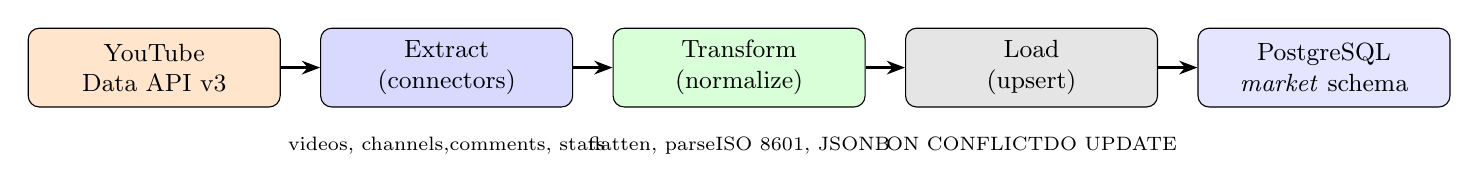
\begin{tikzpicture}[
    node distance=0.6cm and 0.5cm,
    box/.style={draw, rounded corners=4pt, fill=#1, minimum width=3.2cm,
                minimum height=1.0cm, align=center, font=\small},
    arr/.style={-Stealth, thick}
]
\node[box=orange!20] (api) {YouTube\\Data API v3};
\node[box=blue!15, right=of api] (extract) {Extract\\(connectors)};
\node[box=green!15, right=of extract] (transform) {Transform\\(normalize)};
\node[box=gray!20, right=of transform] (load) {Load\\(upsert)};
\node[box=blue!10, right=of load] (db) {PostgreSQL\\\textit{market} schema};

\draw[arr] (api) -- (extract);
\draw[arr] (extract) -- (transform);
\draw[arr] (transform) -- (load);
\draw[arr] (load) -- (db);

\node[font=\scriptsize, below=0.25cm of extract] {videos, channels,\\comments, stats};
\node[font=\scriptsize, below=0.25cm of transform] {flatten, parse\\ISO 8601, JSONB};
\node[font=\scriptsize, below=0.25cm of load] {ON CONFLICT\\DO UPDATE};
\end{tikzpicture}
\caption{Market ETL pipeline: data flows from the YouTube Data API~v3 through extraction, normalization, and idempotent loading into PostgreSQL.}
\label{fig:etl_pipeline}
\end{figure}

\textbf{Extraction.} Four specialized connectors implement the extraction logic: \texttt{video.py} retrieves video metadata using \texttt{videos.list()} with the \texttt{snippet}, \texttt{contentDetails}, and \texttt{statistics} parts; \texttt{channel.py} deduplicates and fetches channel records from video rows; \texttt{comment.py} paginates comment threads; and \texttt{video\_stats.py} records point-in-time engagement snapshots. Trending content is retrieved via the \texttt{chart=mostPopular} parameter with configurable \texttt{regionCode} and \texttt{videoCategoryId} filters.

\textbf{Transformation.} Raw API responses are normalized into flat dictionaries with explicit field selection, ISO~8601 duration parsing via \texttt{isoparse()}, and JSONB preservation of the full raw snippet for schema-forward compatibility.

\textbf{Loading.} PostgreSQL \texttt{INSERT … ON CONFLICT DO UPDATE} statements provide idempotent upserts: repeated ingestion runs update existing records without duplication. Batch inserts are wrapped in database transactions to ensure atomicity.

\textbf{Orchestration.} The \texttt{IngestionService} class composes the three stages into four high-level operations: trending full sync, search-based sync, direct video ID sync, and per-video comment sync. These are exposed as CLI commands via the Typer-based \texttt{cip} entry point and as REST endpoints via the \texttt{/market/sync/} router.

%--------------------------------------------------
\section{Market Analytics and Insights}

The analytics module aggregates stored engagement data into actionable KPIs exposed through the \texttt{/market/overview} and \texttt{/market/charts/} endpoints.

\textbf{KPI aggregation.} The overview endpoint returns total video count, channel count, comment count, and total views computed as the sum of the most recent engagement snapshot for each video, using a window-function subquery to select \texttt{MAX(snapshot\_time)} per video.

\textbf{Chart data.} Three chart endpoints support the React dashboard: (i)~top ten videos by view count; (ii)~daily aggregated views over a rolling 30-day window; and (iii)~video count per category as a percentage breakdown.

\textbf{Trend keyword extraction.} The \texttt{/insights/trending-keywords} endpoint extracts high-frequency terms from the titles of videos with above-average views in a configurable time window (default: 7 days). Titles are tokenized, lowercased, and filtered for tokens of three or more characters. The resulting keyword list is injected into LLM description generation prompts to improve discoverability without manual SEO research.

%--------------------------------------------------
\section{Video-to-Shorts Pipeline}

The Video-to-Shorts pipeline is the most computationally intensive module of the platform. It takes a single video file as input and produces a ranked set of short-form video clips suitable for publication on vertical format platforms (YouTube Shorts, Instagram Reels, TikTok). The pipeline operates in six sequential stages, as illustrated in Figure~\ref{fig:shorts_pipeline}.

\begin{figure}[H]
\centering
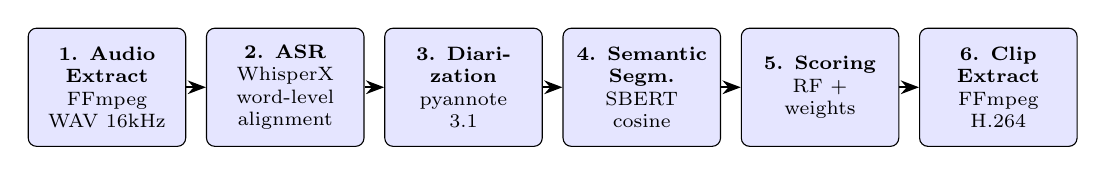
\begin{tikzpicture}[
    node distance=0.35cm and 0.25cm,
    stage/.style={draw, rounded corners=3pt, fill=blue!10,
                  minimum width=2.0cm, minimum height=1.5cm,
                  align=center, font=\scriptsize},
    arr/.style={-Stealth, thick}
]
\node[stage] (s1) {\textbf{1. Audio}\\\textbf{Extract}\\FFmpeg\\WAV 16kHz};
\node[stage, right=of s1] (s2) {\textbf{2. ASR}\\WhisperX\\word-level\\alignment};
\node[stage, right=of s2] (s3) {\textbf{3. Diari-}\\\textbf{zation}\\pyannote\\3.1};
\node[stage, right=of s3] (s4) {\textbf{4. Semantic}\\\textbf{Segm.}\\SBERT\\cosine};
\node[stage, right=of s4] (s5) {\textbf{5. Scoring}\\RF +\\weights};
\node[stage, right=of s5] (s6) {\textbf{6. Clip}\\\textbf{Extract}\\FFmpeg\\H.264};

\draw[arr] (s1) -- (s2);
\draw[arr] (s2) -- (s3);
\draw[arr] (s3) -- (s4);
\draw[arr] (s4) -- (s5);
\draw[arr] (s5) -- (s6);
\end{tikzpicture}
\caption{Six-stage Video-to-Shorts pipeline. The scoring stage combines four weighted factors into a composite clip score.}
\label{fig:shorts_pipeline}
\end{figure}

\subsection*{Stage 1: Audio extraction}

FFmpeg extracts the audio track from the input video and converts it to a 16kHz mono WAV file, the format required by the ASR and audio analysis components. Video duration is queried via \texttt{ffprobe} for progress computation.

\subsection*{Stage 2: Automatic speech recognition}

Transcription is performed using WhisperX \cite{bain2023whisperx}, which extends OpenAI Whisper \cite{radford2023whisper} with forced phoneme alignment. This produces word-level timestamps with higher precision than the default Whisper output, enabling accurate clip boundary placement at sentence boundaries. The model size is configurable via the \texttt{WHISPER\_MODEL} environment variable (default: \texttt{small}); larger models improve accuracy at the cost of inference time.

\subsection*{Stage 3: Speaker diarization}

Speaker assignment is performed using the \texttt{pyannote/speaker-diarization-3.1} model \cite{bredin2021pyannote} accessed via Hugging Face Hub (requires an \texttt{HF\_TOKEN} environment variable). Each transcript segment is assigned a speaker label by matching its midpoint timestamp to the diarization output. Diarization is optional: if the Hugging Face token is unavailable or inference fails, the pipeline continues without speaker information.

\subsection*{Stage 4: Semantic segmentation}

Candidate clip boundaries are identified using cosine similarity between consecutive SBERT sentence embeddings \cite{reimers2019sbert}. A similarity score below a threshold of 0.35 is interpreted as a topic shift, triggering a boundary. Segments between consecutive boundaries are merged into candidate clips, with duration constraints enforced via configurable parameters (\texttt{MIN\_CLIP\_DURATION}, \texttt{MAX\_CLIP\_DURATION}, \texttt{TARGET\_CLIP\_DURATION}). This approach detects thematic transitions without requiring visual features, enabling CPU-only operation.

\subsection*{Stage 5: Multi-factor scoring}

Each candidate clip is scored across four independent dimensions, combined into a weighted composite score $S$:

\begin{equation}
S = w_{\text{sh}} \cdot s_{\text{sh}} + w_{\text{sem}} \cdot s_{\text{sem}} + w_{\text{hook}} \cdot s_{\text{hook}} + w_{\text{spk}} \cdot s_{\text{spk}}
\label{eq:scoring}
\end{equation}

where the weight vector $(w_{\text{sh}}, w_{\text{sem}}, w_{\text{hook}}, w_{\text{spk}}) = (0.50, 0.20, 0.15, 0.15)$ is configurable via environment variables and the React UI. The four scoring components are:

\begin{itemize}
\item \textbf{Shortability score} ($s_{\text{sh}}$, weight~0.50): A Random Forest classifier \cite{breiman2001rf} trained on 12 audio and semantic features (RMS energy, zero-crossing rate, spectral centroid, silence ratio, speech rate, semantic similarity, clip position, duration, speaker change count, question mark presence, exclamation mark presence, hook score). The model produces a continuous shortability probability.
\item \textbf{Semantic score} ($s_{\text{sem}}$, weight~0.20): Cosine similarity between the clip embedding and the full video transcript embedding, measuring the informativeness of the segment relative to the whole.
\item \textbf{Hook score} ($s_{\text{hook}}$, weight~0.15): A rule-based detector matching language-specific regex patterns for contradiction phrases, announcement structures, and interrogative forms. Returns a score in $[0,1]$ based on pattern count and type.
\item \textbf{Speaker change score} ($s_{\text{spk}}$, weight~0.15): A normalized measure of speaker transitions within the clip boundaries, rewarding conversational dynamics that correlate with engagement.
\end{itemize}

Audio features are extracted using librosa \cite{mcfee2015librosa} applied to the WAV segment corresponding to each candidate clip.

\subsection*{Stage 6: Clip extraction}

The top-$N$ candidates (configurable, default $N=5$) are extracted as MP4 files using FFmpeg with libx264 video encoding and AAC audio, with 0.5-second fade-in and fade-out effects. A vertical (9:16) variant is produced for each clip via a center-crop filter scaled to $1080 \times 1920$~pixels, suitable for publication on Shorts and Reels.

An optional title generation step invokes the Anthropic Claude API with the clip transcript and hook type as context, producing a platform-optimized title (maximum 60~characters) and five relevant hashtags.

Job progress is tracked at each stage transition (0.05 $\rightarrow$ 0.15 $\rightarrow$ 0.30 $\rightarrow$ 0.45 $\rightarrow$ 0.55 $\rightarrow$ 0.70 $\rightarrow$ 0.85 $\rightarrow$ 1.00) and persisted in the \texttt{app.jobs} table, enabling real-time progress monitoring from the frontend.

%--------------------------------------------------
\section{Subtitle Generation Pipeline}

The subtitle pipeline uses faster-whisper \cite{fasterwhisper} (CTranslate2-quantized Whisper, default model \texttt{large-v2}) to generate SRT subtitle files from uploaded video assets.

Long videos are processed in 10-minute audio chunks with a 5-second overlap between consecutive chunks, preventing ASR context loss at segment boundaries. After independent transcription of each chunk, segment timestamps are normalized and overlapping regions are deduplicated before SRT serialization.

Generated subtitle artefacts are stored in the \texttt{studio.subtitle\_artifacts} table, with paths to both the SRT file and an optional FFmpeg-processed video with burned-in subtitles (\texttt{subtitles} filter). Transcript segments are written to \texttt{studio.transcript\_segments} with language annotation (BCP-47 code), enabling downstream reuse by the description generation and Shorts pipeline.

%--------------------------------------------------
\section{Multimodal Description Generation}

The description generation module synthesizes SEO-optimized YouTube descriptions from two information sources: (i)~the video transcript stored in \texttt{studio.transcript\_segments}, and (ii)~trending keyword signals retrieved from the \texttt{/insights/trending-keywords} endpoint.

The generation prompt is structured in three parts: a hook paragraph directive, a key-topics extraction instruction with bullet-point formatting, and a hashtag generation request. Trending keywords are injected into the prompt with an instruction to integrate them naturally into the output. The system prompt establishes the LLM's role as an expert in YouTube SEO and platform content strategy.

Prompts are localized for nine languages (Spanish, English, French, German, Italian, Portuguese, Japanese, Korean, Chinese) to enable market-specific description generation without translation post-processing. Generated descriptions are stored in \texttt{studio.generated\_descriptions} with the model name and language code, supporting comparison across LLM providers and prompt versions.

The local Ollama backend provides an alternative for privacy-sensitive or offline deployments, with negligible code change at the application layer due to the \texttt{GenerationPort} interface abstraction.

%--------------------------------------------------
\section{REST API and Frontend}

The FastAPI application organizes endpoints into four routers: \texttt{/market} (ingestion and analytics), \texttt{/studio} (asset management and pipeline execution), \texttt{/jobs} (status polling and clip download), and \texttt{/insights} (keyword extraction). All inputs are validated via Pydantic schemas; all responses include structured JSON payloads. CORS is configured to accept all origins during development.

Long-running operations (subtitle generation, shorts pipeline, description generation) are dispatched as \texttt{BackgroundTask} instances: the endpoint creates the job record, returns the job UUID immediately, and the task updates progress asynchronously. Clients poll \texttt{GET /jobs/\{job\_id\}} until \texttt{status} reaches \texttt{completed} or \texttt{failed}.

The React frontend implements two primary views: a \textit{Market} tab with KPI cards, sortable video table, and three Recharts visualizations (bar chart, line chart, pie chart); and a \textit{Studio} tab with drag-and-drop asset upload, asset selection sidebar, and a detail panel exposing transcript preview, generated description, job status progress bar, and the Shorts clip grid. Score weight sliders in the \textit{ShortsModal} component allow users to re-score previously generated candidates with updated weights, invoking the \texttt{POST /assets/\{id\}/shorts/rescore} endpoint without rerunning the full pipeline.

%--------------------------------------------------
\section{Economic Evaluation of the Project}

\subsection{Development Costs}

The project was developed over approximately 14 weeks as a single-developer effort. Table~\ref{tab:dev_costs} estimates the development cost based on average junior data scientist and frontend developer rates in Spain (approximately €20–25 per hour).

\begin{table}[H]
\centering
\caption{Estimated development cost breakdown.}
\label{tab:dev_costs}
\begin{tabular}{@{}lrrl@{}}
\toprule
\textbf{Area} & \textbf{Hours} & \textbf{Rate (€/h)} & \textbf{Cost (€)} \\
\midrule
Backend architecture and API          & 110 & 22 & 2,420 \\
Machine learning pipelines (Shorts, ASR) & 140 & 25 & 3,500 \\
Database design and migrations        &  40 & 20 & 800   \\
NLP and LLM integration               &  60 & 22 & 1,320 \\
Frontend (React SPA)                  &  80 & 20 & 1,600 \\
Testing, integration, documentation  &  50 & 15 & 750   \\
\midrule
\textbf{Total}                        & \textbf{480} & & \textbf{10,390} \\
\bottomrule
\end{tabular}
\end{table}

The 480 estimated hours align with a 14-week project at approximately 34 productive hours per week, which is consistent with part-time academic development alongside coursework.

\subsection{Infrastructure Costs}

Table~\ref{tab:infra_costs} shows the estimated monthly operational costs for a production deployment on AWS, sized for a small-scale SaaS service handling up to 200 active users.

\begin{table}[H]
\centering
\caption{Estimated monthly infrastructure costs (small-scale production deployment).}
\label{tab:infra_costs}
\begin{tabular}{@{}llrl@{}}
\toprule
\textbf{Component} & \textbf{Service} & \textbf{Monthly Cost (€)} & \textbf{Notes} \\
\midrule
PostgreSQL database      & AWS RDS t3.micro        & 18    & 1 vCPU, 1 GB RAM \\
API server               & AWS EC2 t3.small        & 16    & 2 vCPU, 2 GB RAM \\
GPU compute (Shorts)     & EC2 g4dn.xlarge (on-demand) & 26 & 20 h/month estimated \\
Video file storage       & AWS S3 (100 GB)         & 2.30  & €0.023/GB/month \\
Data transfer            & AWS egress (50 GB)      & 4.50  & €0.09/GB \\
\midrule
\textbf{Total monthly}   &                         & \textbf{66.80} & \\
\bottomrule
\end{tabular}
\end{table}

GPU instances are provisioned on-demand and terminated after job completion, ensuring that compute costs scale with actual Shorts pipeline usage rather than being incurred continuously.

\subsection{Third-Party API Costs}

\begin{table}[H]
\centering
\caption{Estimated monthly third-party API costs for 100 active video operations.}
\label{tab:api_costs}
\begin{tabular}{@{}lll@{}}
\toprule
\textbf{Service} & \textbf{Operation} & \textbf{Monthly Cost (€)} \\
\midrule
YouTube Data API v3  & Trending sync (free quota: 10,000 units/day) & 0.00 \\
Anthropic Claude API & 100 descriptions $\times$ $\sim$500 tokens avg. & $\approx$ 1.50 \\
Hugging Face Hub     & Model downloads (cached after first use)      & 0.00 \\
\midrule
\textbf{Total}       &                                               & $\approx$ \textbf{1.50} \\
\bottomrule
\end{tabular}
\end{table}

The YouTube Data API free quota is sufficient for small-to-medium monitoring workloads. Claude API costs remain negligible at this scale; at 1,000 operations per month, the estimated cost would be approximately €15.

\subsection{Revenue Model and Break-Even Analysis}

The platform is amenable to a SaaS subscription model targeting independent YouTube creators with more than 10,000 subscribers — a segment estimated at approximately 2 million globally. Three pricing tiers are proposed:

\begin{itemize}
\item \textbf{Basic} (€29/month): Market analytics dashboard + subtitle generation.
\item \textbf{Pro} (€59/month): Basic + Video-to-Shorts pipeline (up to 20 videos/month).
\item \textbf{Studio} (€99/month): Pro + description generation + API access.
\end{itemize}

Table~\ref{tab:breakeven} presents the break-even analysis at three user-count scenarios.

\begin{table}[H]
\centering
\caption{Break-even analysis at different subscriber volumes (Pro tier, €59/month).}
\label{tab:breakeven}
\begin{tabular}{@{}lrrrr@{}}
\toprule
\textbf{Users} & \textbf{Revenue (€/mo.)} & \textbf{Infra (€/mo.)} & \textbf{Profit (€/mo.)} & \textbf{Dev. recovery} \\
\midrule
20  & 1,180 & 100  & 1,080 & $\approx$ 10 months \\
50  & 2,950 & 200  & 2,750 & $\approx$ 4 months \\
100 & 5,900 & 350  & 5,550 & $\approx$ 2 months \\
\bottomrule
\end{tabular}
\end{table}

Infrastructure costs scale sub-linearly with user count: additional users primarily increase storage and API call volume, while the database and API server remain within the same instance tier up to approximately 200 concurrent users.

\subsection{Value Proposition for End Users}

Beyond the provider-side economics, the platform delivers measurable time savings to content creators. Table~\ref{tab:creator_value} estimates the production time saved per video across the three main automated tasks.

\begin{table}[H]
\centering
\caption{Estimated production time savings per video for a YouTube creator.}
\label{tab:creator_value}
\begin{tabular}{@{}lll@{}}
\toprule
\textbf{Task} & \textbf{Manual time} & \textbf{Platform time} \\
\midrule
Subtitle creation and synchronization & 60–90 min & 5–10 min (review only) \\
Short-form clip selection and editing & 90–150 min & 10–15 min (review only) \\
SEO description writing               & 20–30 min & 2–5 min (review only)  \\
\midrule
\textbf{Total per video}              & $\approx$ 3–4.5 h & $\approx$ 20–30 min \\
\bottomrule
\end{tabular}
\end{table}

For a creator producing four videos per month at an effective hourly rate of €25, the platform generates approximately €300–€400 in recovered productive time per month against a subscription cost of €29–€59/month, yielding a user-side ROI exceeding 500\%.

\subsection{Viability Assessment}

The economic analysis demonstrates that the project is viable as a deployable SaaS product. Development costs are within the range of a small startup MVP (approximately €10,000). Monthly operational costs at small scale remain below €70, and a break-even subscriber count of fewer than 20 users at the Pro tier makes the revenue target achievable. The primary barrier to commercialization is not technical feasibility or cost structure, but market acquisition — acquiring early adopters requires distribution channels such as creator communities, YouTube-focused newsletters, and direct outreach to mid-tier channels.

From a research perspective, the platform demonstrates that a single developer can implement a production-quality AI-assisted content pipeline within an academic project timeframe, using exclusively open-source ML frameworks and affordable cloud infrastructure.


%==========================================================
\chapter{Results}

This chapter presents the experimental evaluation of the developed platform modules. Results are organized by pipeline component, assessing both computational performance and output quality.

Figures must be cited and explained in the text, such as Figure~\ref{fig:my_label}, where the error is shown as a function of distance in arbitrary units. All plots must include axis labels.

\begin{figure}[!htbp]
    \centering
    \includegraphics[width=7truecm]{Rplotmanh.png}
    \caption{Error as a function of distance in arbitrary units.}
    \label{fig:my_label}
\end{figure}

\chapter{Conclusions and Future Works}

This chapter must include:
\begin{itemize}
\item A description of the conclusions of the work:
\begin{itemize}
    \item Once the results have been obtained, what conclusions are drawn?
    \item Are these results as expected? Or have they been surprising? Why?
\end{itemize}
\item A critical reflection on the achievement of the objectives initially set:
\begin{itemize}
    \item Have all objectives been achieved? If not, why?
\end{itemize}
\item A critical analysis of the monitoring of planning and methodology throughout the project:
\begin{itemize}
    \item Has the schedule been followed?
    \item Has the planned methodology been adequate?
    \item Has it been necessary to introduce changes to ensure the success of the work? Why?
\end{itemize}
\item From the impacts foreseen in \ref{s:etic}, an evaluation of whether negative impacts have been mitigated or positive impacts have been achieved.
\item If unforeseen impacts have appeared, an evaluation of how they have been managed.
\item The future lines of work that have not been explored and remain pending.
\end{itemize}

\chapter{Glossary}

\begin{description}
\item[API] Application Programming Interface. A set of protocols enabling communication between software components.
\item[ASR] Automatic Speech Recognition. The task of converting spoken audio to text.
\item[BCP-47] Internet standard for language tags (e.g., \texttt{es}, \texttt{en-US}).
\item[CTR] Click-Through Rate. The ratio of clicks to impressions for a video thumbnail.
\item[ETL] Extract-Transform-Load. A standard data integration pattern.
\item[GPU] Graphics Processing Unit. A processor suited to parallel matrix computation, used here for ML model inference.
\item[KPI] Key Performance Indicator. A quantitative metric used to evaluate performance.
\item[LLM] Large Language Model. A neural language model with billions of parameters trained on large text corpora.
\item[ORM] Object-Relational Mapping. A technique for translating between database relations and programming language objects.
\item[SBERT] Sentence-BERT. A modification of BERT producing semantically rich sentence-level embeddings.
\item[SEO] Search Engine Optimization. Practices aimed at improving content discoverability.
\item[SRT] SubRip Text. A subtitle file format containing timestamped text segments.
\item[SaaS] Software as a Service. A software delivery model where applications are hosted and accessed over the internet.
\item[VOD] Video-on-Demand. A media distribution model allowing users to access video content on request.
\item[WSL] Windows Subsystem for Linux. A compatibility layer enabling Linux execution on Windows.
\end{description}


\bibliographystyle{IEEEtran}
\bibliography{references}

\newpage
\appendix

\section*{Appendix A: Environment Configuration}

The platform is configured entirely through environment variables loaded via Pydantic Settings. Table~\ref{tab:env_vars} documents the principal configuration parameters.

\begin{table}[H]
\centering
\caption{Principal environment variables and their default values.}
\label{tab:env_vars}
\begin{tabular}{@{}llp{5cm}@{}}
\toprule
\textbf{Variable} & \textbf{Default} & \textbf{Description} \\
\midrule
\texttt{DATABASE\_URL}       & —                   & PostgreSQL connection string \\
\texttt{YT\_API\_KEY}        & —                   & YouTube Data API v3 key \\
\texttt{ANTHROPIC\_API\_KEY} & —                   & Anthropic Claude API key \\
\texttt{HF\_TOKEN}           & —                   & Hugging Face access token \\
\texttt{WHISPER\_MODEL}      & \texttt{small}      & Whisper model size \\
\texttt{NUM\_CLIPS}          & \texttt{5}          & Clips to extract per video \\
\texttt{MIN\_CLIP\_DURATION} & \texttt{5.0}        & Minimum clip duration (s) \\
\texttt{MAX\_CLIP\_DURATION} & \texttt{30.0}       & Maximum clip duration (s) \\
\texttt{SCORE\_SHORTABILITY} & \texttt{0.50}       & Weight for shortability score \\
\texttt{SCORE\_SEMANTIC}     & \texttt{0.20}       & Weight for semantic score \\
\texttt{SCORE\_HOOK}         & \texttt{0.15}       & Weight for hook score \\
\texttt{SCORE\_SPEAKER\_CHANGE} & \texttt{0.15}    & Weight for speaker change score \\
\texttt{EMBEDDING\_MODEL}    & \texttt{all-mpnet-base-v2} & SBERT model identifier \\
\texttt{CIP\_DATA\_DIR}      & \texttt{./data}     & Root directory for file artefacts \\
\bottomrule
\end{tabular}
\end{table}

\end{document}
